\PassOptionsToPackage{table, dvipsnames}{xcolor}

\documentclass[a4paper,twoside,12pt]{article}

%-------------------------------------------------------------------------------
% CONFIGURAZIONE BASE DEL DOCUMENTO
%-------------------------------------------------------------------------------
\usepackage[T1]{fontenc}
\usepackage[utf8]{inputenc}
\usepackage[english]{babel}
\usepackage{amssymb}
\usepackage{amsmath}

%-------------------------------------------------------------------------------
% PACKAGE PER GRAFICA E IMMAGINI
%-------------------------------------------------------------------------------
\usepackage{multirow}
\usepackage{geometry}
\geometry{a4paper, margin=2.5cm}
\usepackage{graphicx}
\usepackage{afterpage}
\usepackage{placeins}
\usepackage{tikz}
\usetikzlibrary{positioning, shapes.geometric, arrows.meta, shadows}
\usepackage{listings}
\usepackage[font=small,skip=10pt]{caption}
\usepackage{subcaption}
\usepackage{booktabs} 
\usepackage{longtable} 
\usepackage{float} 
\usepackage{siunitx} 
\usepackage{makecell}
\usepackage{fancyhdr}
\usepackage{setspace}

%-------------------------------------------------------------------------------
% PACKAGE PER COLORI E TABELLE
%-------------------------------------------------------------------------------
\usepackage[table]{xcolor}

%-------------------------------------------------------------------------------
% PACKAGE PER IPERTESTI E RIFERIMENTI
%-------------------------------------------------------------------------------
\usepackage{hyperref}
\hypersetup{
    pdfkeywords={Process Mining, BPI Challenge 2012, Petri Net, LLM, pm4py},
    colorlinks=true,
    linkcolor=black,
    citecolor=Green,
    urlcolor=NavyBlue,
    filecolor=magenta,
    bookmarksnumbered=true,
    breaklinks=true,
    pdfpagemode=UseOutlines,
    pdfstartview=FitH,
    unicode=true
}

%-------------------------------------------------------------------------------
% IMPOSTAZIONI DI FORMATTAZIONE
%-------------------------------------------------------------------------------
\linespread{1.25}
\onehalfspacing

% Listings configuration for Python code
\lstset{
    language=Python,
    basicstyle=\ttfamily\footnotesize,
    keywordstyle=\color{blue}\bfseries,
    stringstyle=\color{red},
    commentstyle=\color{green!60!black},
    numbers=left,
    numberstyle=\tiny\color{gray},
    stepnumber=1,
    numbersep=5pt,
    backgroundcolor=\color{gray!10},
    showspaces=false,
    showstringspaces=false,
    showtabs=false,
    frame=single,
    rulecolor=\color{black},
    tabsize=4,
    captionpos=b,
    breaklines=true,
    breakatwhitespace=false,
    escapeinside={\%*}{*)},
    morekeywords={pm4py, streamlit, pandas}
}

%-------------------------------------------------------------------------------
% DEFINIZIONI PER IL FRONTESPIZIO
%-------------------------------------------------------------------------------
\def\dept{DEPARTMENT OF COMPUTER SCIENCE}
\def\course{MASTER'S DEGREE IN COMPUTER SCIENCE}
\def\reporttitle{Process Mining Analysis on the BPI Challenge 2012 Dataset}
\def\reportsubtitle{Discovery, Evaluation, and Optimization of Process Models with Large Language Models Integration}
\def\studentname{Fabio Zippo}
\def\supervisorname{Prof.ssa Berardina De Carolis}
\def\subject{FORMAL METHODS}
\def\academicyear{2024 - 2025}

% Header and Footer
\pagestyle{fancy}
\fancyhf{}
\rhead{Process Mining - BPI Challenge 2012}
\lhead{Formal Methods}
\cfoot{\thepage}

%-------------------------------------------------------------------------------
% INIZIO DEL DOCUMENTO
%-------------------------------------------------------------------------------
\begin{document}

%-------------------------------------------------------------------------------
% FRONTESPIZIO
%-------------------------------------------------------------------------------
\begin{titlepage}
	\begin{tikzpicture}[remember picture,overlay]
		\centering
		\node[yshift=-5cm] (logo) at (current page.north) {
\includegraphics[width=0.6\linewidth]{logo.png}};
		\node[text width=50em,yshift=0.5cm, align=center, below=of logo](dipartimento){\normalsize \dept};
		\node[text width=40em, align=center, yshift=0.75cm, below=of dipartimento](coursename){\normalsize \course};
		\node[text width=35em, align=center, yshift=1.2cm, below=of coursename](line){\par\noindent\rule{\textwidth}{0.4pt}};
		\node[text width=40em, align=center, yshift=0.55cm, below=of line](subjectline){\normalsize PROJECT REPORT FOR \\ \subject};
		
		\node[text width=40em, align=center, yshift=-0.3cm, below=of subjectline](title){\bfseries \parbox{14cm}{\fontsize{18pt}{22pt}\selectfont \centering \reporttitle\par}};
		
		\node[text width=40em, align=center, yshift=0.3cm, below=of title](subtitle){\large \reportsubtitle};
		
		\node[text width=35em, align=left, yshift=-0.8cm, below=of subtitle](supervisortit){\normalsize \textbf{SUPERVISOR:}};
		\node[text width=35em, align=left, yshift=1cm, below=of supervisortit](supervisor){\large \supervisorname};
		
		\node[text width=35em, align=right, yshift=-0.8cm, below=of subtitle](studenttit){\normalsize \textbf{STUDENT:}};
		\node[text width=35em, align=right, yshift=1cm, below=of studenttit](student){\large \studentname};
		
		\node[text width=35em, align=center, yshift=-2.5cm, below=of student](line2){\par\noindent\rule{\textwidth}{0.4pt}};
		
		\node[text width=50em, align=center, yshift=0.5cm, below=of line2](year){\large ACADEMIC YEAR \academicyear};
	\end{tikzpicture}
\end{titlepage}

%============================================
% ABSTRACT
%============================================
\newpage
\begin{abstract}
This work presents a comprehensive Process Mining project applied to the BPI Challenge 2012 dataset, which represents a real-world loan application management process at a Dutch financial institution. The main objective was to extract, analyze, and compare process models using three fundamental algorithms: Alpha Miner, Heuristic Miner, and Inductive Miner.

The developed system consists of three main components: (i) an offline mining pipeline for automatic model discovery and quality metrics computation (fitness, precision, simplicity, generalization); (ii) a context generation module for integration with Large Language Models (LLM), enabling advanced analysis through automated reasoning; (iii) an interactive Streamlit-based dashboard that allows results visualization, bottleneck analysis, and interaction with an AI assistant for predicting the next activities in the process.

The results show that the Heuristic Miner with a dependency threshold of 0.5 and the Inductive Miner with a noise threshold of 0.2 produce models with fitness exceeding 90\%, while the Alpha Miner exhibits significant limitations in handling complex logs with loops and concurrent behaviors. The bottleneck analysis identified that the most critical transitions involve manual request completion activities, with average waiting times up to 128 hours. The integration with GPT-3.5-turbo demonstrated the feasibility of intelligent decision support systems for business process optimization.

\textbf{Keywords:} Process Mining, BPI Challenge 2012, Petri Net, Alpha Miner, Heuristic Miner, Inductive Miner, Large Language Models, Streamlit, pm4py.
\end{abstract}

\newpage
\tableofcontents
\newpage

%============================================
% INTRODUCTION
%============================================
\section{Introduction}

\subsection{Context and Motivation}

Process Mining represents an emerging discipline that lies at the intersection between Data Mining and Business Process Management (BPM). The fundamental objective is to extract knowledge from so-called \textit{event logs}, digital records of activities performed within enterprise information systems, to discover, monitor, and improve real processes.

In an increasingly data-driven business context, the ability to understand how processes are actually executed (as opposed to how they were designed) becomes crucial for operational optimization. The BPI Challenge 2012 dataset, released as part of the Business Process Intelligence Challenge, represents a reference benchmark in the scientific community, containing real data from a loan application management process at a Dutch financial institution.

\subsection{Project Objectives}

The main objectives of this project are:

\begin{enumerate}
    \item \textbf{Process Discovery}: Apply and compare three automatic process discovery algorithms (Alpha Miner, Heuristic Miner, Inductive Miner) to generate formal models in the form of Petri Nets.
    
    \item \textbf{Conformance Checking}: Evaluate the quality of discovered models through established metrics such as fitness, precision, simplicity, and generalization.
    
    \item \textbf{Performance Analysis}: Identify process bottlenecks by analyzing transition times between activities.
    
    \item \textbf{LLM Integration}: Develop an automated reasoning system based on Large Language Models to generate management reports and optimization suggestions.
    
    \item \textbf{Interactive Dashboard}: Create an interactive user interface for results visualization and interaction with an AI assistant.
\end{enumerate}

\subsection{Document Structure}

The document is organized as follows: Section 2 presents the theoretical background on Process Mining and the algorithms used; Section 3 describes the BPI Challenge 2012 dataset; Section 4 illustrates the system architecture and implementation; Section 5 presents the experimental results; Section 6 discusses the integration with Large Language Models; Section 7 details the automated LLM reasoning pipeline; finally, Section 8 concludes the work with final considerations and possible future developments.

%============================================
% THEORETICAL BACKGROUND
%============================================
\section{Theoretical Background}

\subsection{Process Mining: Definition and Types}

Process Mining is based on the analysis of \textit{event logs}, data structures that record the execution of activities within a process. Formally, an event log $L$ is defined as a multiset of traces, where each trace $\sigma = \langle e_1, e_2, \ldots, e_n \rangle$ is a sequence of events. Each event $e$ is characterized by at least three fundamental attributes:

\begin{itemize}
    \item \textbf{Case ID}: unique identifier of the process instance
    \item \textbf{Activity}: name of the executed activity
    \item \textbf{Timestamp}: timestamp of the execution
\end{itemize}

The three main types of Process Mining are:

\begin{enumerate}
    \item \textbf{Process Discovery}: automatic discovery of a process model from the event log
    \item \textbf{Conformance Checking}: verification of conformance between a model and observed behavior
    \item \textbf{Enhancement}: improvement of an existing model with additional information
\end{enumerate}

\subsection{Petri Nets as a Representation Formalism}

Petri Nets constitute the most widespread mathematical formalism for representing process models in the context of Process Mining. A Petri Net is a tuple $PN = (P, T, F, M_0)$ where:

\begin{itemize}
    \item $P$ is a finite set of \textit{places}
    \item $T$ is a finite set of \textit{transitions}
    \item $F \subseteq (P \times T) \cup (T \times P)$ is the flow relation
    \item $M_0: P \rightarrow \mathbb{N}$ is the initial marking
\end{itemize}

Petri Nets allow modeling fundamental constructs such as sequence, exclusive choice (XOR-split), parallelism (AND-split), and synchronization.

\subsection{Process Discovery Algorithms}

\subsubsection{Alpha Miner}

The Alpha Miner, introduced by van der Aalst et al. (2004), is one of the pioneering algorithms for automatic process discovery. The algorithm analyzes the ordering relations between activities in the event log to construct a Petri Net. The fundamental relations are:

\begin{itemize}
    \item $a >_L b$: $a$ is directly followed by $b$ in at least one trace
    \item $a \rightarrow_L b$: $a >_L b$ and $\neg(b >_L a)$ (causality)
    \item $a \parallel_L b$: $a >_L b$ and $b >_L a$ (parallelism)
    \item $a \#_L b$: $\neg(a >_L b)$ and $\neg(b >_L a)$ (no direct relation)
\end{itemize}

\textbf{Limitations}: The Alpha Miner does not correctly handle loops of length one or two, non-local behaviors, and noisy logs.

\subsubsection{Heuristic Miner}

The Heuristic Miner, proposed by Weijters et al. (2006), extends the Alpha Miner approach by introducing frequency-based metrics to handle noise in data. The algorithm calculates a \textit{dependency measure} between pairs of activities:

\begin{equation}
    \text{dependency}(a, b) = \frac{|a >_L b| - |b >_L a|}{|a >_L b| + |b >_L a| + 1}
\end{equation}

Dependency relations are filtered through a configurable threshold (\textit{dependency threshold}), allowing spurious relations caused by noise to be ignored.

\subsubsection{Inductive Miner}

The Inductive Miner, introduced by Leemans et al. (2013), adopts a divide-and-conquer approach guaranteeing the generation of \textit{sound} models (free from deadlocks and livelocks). The algorithm constructs a \textit{process tree} through:

\begin{enumerate}
    \item Identification of a \textit{cut} that partitions the activities
    \item Recursive application to the resulting sub-logs
    \item Final conversion of the process tree to a Petri Net
\end{enumerate}

The \textit{noise threshold} parameter allows filtering of infrequent behaviors.

\subsection{Model Quality Metrics}

The quality of a process model is evaluated through four dimensions:

\begin{enumerate}
    \item \textbf{Fitness}: measures the model's ability to reproduce the behavior observed in the event log. A fitness of 1.0 indicates that all traces can be replicated by the model.
    
    \item \textbf{Precision}: measures the model's ability to disallow unobserved behaviors. A model that allows any sequence (``flower model'') has low precision.
    
    \item \textbf{Simplicity}: evaluates the structural complexity of the model, preferring simpler models according to Occam's razor principle.
    
    \item \textbf{Generalization}: estimates the model's ability to generalize to unobserved but plausible traces.
\end{enumerate}

%============================================
% DATASET
%============================================
\section{Dataset: BPI Challenge 2012}

\subsection{Process Description}

The BPI Challenge 2012 dataset contains the event log of a personal loan application management process at a Dutch financial institution. The process includes several phases:

\begin{enumerate}
    \item \textbf{Submission}: the customer submits a loan application
    \item \textbf{Evaluation}: the institution evaluates the application
    \item \textbf{Offer}: an offer is generated and sent to the customer
    \item \textbf{Negotiation}: possible interaction to modify the conditions
    \item \textbf{Final Decision}: approval or rejection of the loan
\end{enumerate}

\subsection{Log Characteristics}

\begin{table}[H]
\centering
\begin{tabular}{lr}
\toprule
\textbf{Characteristic} & \textbf{Value} \\
\midrule
Total number of cases & 13,087 \\
Total number of events & 164,506 \\
Distinct activities & $\sim$36 \\
Time period & October 2011 - March 2012 \\
\bottomrule
\end{tabular}
\caption{Main statistics of the BPI Challenge 2012 dataset}
\label{tab:dataset_stats}
\end{table}

\subsection{Activity Naming Convention}

Activities in the dataset follow a specific naming convention:

\begin{itemize}
    \item \textbf{A\_*}: automated system activities (e.g., \texttt{A\_SUBMITTED}, \texttt{A\_APPROVED}, \texttt{A\_DECLINED})
    \item \textbf{W\_*}: manual work items requiring human intervention (e.g., \texttt{W\_Completeren aanvraag} - request completion)
    \item \textbf{O\_*}: offer-related events (e.g., \texttt{O\_SENT}, \texttt{O\_SENT\_BACK})
\end{itemize}

\subsection{Lifecycle Transition}

The dataset includes information about the lifecycle of events (\texttt{lifecycle:transition}), with states such as:
\begin{itemize}
    \item \texttt{SCHEDULE}: activity scheduled
    \item \texttt{START}: activity started
    \item \texttt{COMPLETE}: activity completed
\end{itemize}

For process discovery analysis, only events with \texttt{COMPLETE} transition are considered to avoid duplications.

%============================================
% ARCHITECTURE AND IMPLEMENTATION
%============================================
\section{System Architecture and Implementation}

\subsection{Architecture Overview}

The system was designed with a modular architecture consisting of three main components:

\begin{figure}[H]
\centering
\fbox{
\begin{minipage}{0.9\textwidth}
\centering
\vspace{0.5cm}
\textbf{System Architecture}\\[0.5cm]
\begin{tabular}{ccc}
\fbox{\texttt{mine.py}} & $\longrightarrow$ & \fbox{Petri Net + Metrics} \\
$\downarrow$ & & \\
\fbox{\texttt{reasoning.py}} & $\longrightarrow$ & \fbox{LLM Prompt} \\
$\downarrow$ & & \\
\fbox{\texttt{dashboard.py}} & $\longrightarrow$ & \fbox{Web Interface} \\
\end{tabular}
\vspace{0.5cm}
\end{minipage}
}
\caption{System architectural schema}
\end{figure}

\subsection{Component 1: Mining Pipeline (\texttt{mine.py})}

The \texttt{mine.py} module implements the complete pipeline for process discovery and conformance checking.

\subsubsection{Loading and Preprocessing}

\begin{lstlisting}[caption={Loading and preprocessing function}]
def load_convert_and_filter(xes_path, csv_out_path):
    # 1. Load XES file
    log = pm4py.read_xes(xes_path)
    
    # 2. Convert to DataFrame
    df = pm4py.convert_to_dataframe(log)
    df.to_csv(csv_out_path, index=False)
    
    # 3. Filter for COMPLETE lifecycle
    if 'lifecycle:transition' in df.columns:
        df = df[df['lifecycle:transition'].str.upper() == 'COMPLETE']
    
    df = df.sort_values(['case:concept:name', 'time:timestamp'])
    return df
\end{lstlisting}

\subsubsection{Algorithm Implementation}

For each algorithm, the system:
\begin{enumerate}
    \item Applies the discovery algorithm to generate the Petri Net
    \item Saves the graphical visualization of the model
    \item Calculates the four quality metrics via token-based replay
\end{enumerate}

\begin{lstlisting}[caption={Example: Heuristic Miner}]
def heuristic_mining(log_train, log_test, img_name, **params):
    net, im, fm = heuristics_miner.apply(log_train, parameters={
        Parameters.DEPENDENCY_THRESH: params.get('dependency_threshold', 0.5),
        Parameters.AND_MEASURE_THRESH: params.get('and_threshold', 0.65)
    })
    
    # Save visualization
    gviz = pn_visualizer.apply(net, im, fm)
    pn_visualizer.save(gviz, img_name)
    
    # Calculate metrics
    fit = fitness.apply(log_test, net, im, fm)["average_trace_fitness"]
    prec = precision.apply(log_test, net, im, fm)
    simp = simplicity.apply(net)
    gen = generalization.apply(log_test, net, im, fm)
    
    return [fit, prec, simp, gen]
\end{lstlisting}

\subsubsection{Sensitivity Analysis}

The system performs a sensitivity analysis for the Inductive Miner by varying the \texttt{noise\_threshold} parameter with values $\{0.0, 0.2, 0.4, 0.8\}$ to study the impact of noise filtering on model quality.

\subsection{Component 2: LLM Context Generation (\texttt{reasoning.py})}

The \texttt{reasoning.py} module generates a structured prompt for integration with Large Language Models.

\begin{lstlisting}[caption={LLM prompt generation}]
def generate_llm_context():
    # Load data
    df = pd.read_csv(input_file)
    log = pm4py.convert_to_event_log(df)
    
    # Calculate metrics
    net, im, fm = pm4py.discover_petri_net_heuristics(df, dependency_threshold=0.5)
    fitness = pm4py.fitness_token_based_replay(log, net, im, fm)['log_fitness']
    precision = pm4py.precision_token_based_replay(log, net, im, fm)
    
    # Identify bottlenecks
    df_sorted['duration'] = (df_sorted['next_time'] - df_sorted['time:timestamp'])
    edges = df_sorted.groupby(['concept:name', 'next_act'])['duration'].mean()
    bottlenecks = edges.sort_values(ascending=False).head(3)
    
    # Generate structured prompt
    prompt = f"""
    [METRICS]
    - Model Fitness: {fitness:.4f}
    - Model Precision: {precision:.4f}
    - Total Cases: {len(log)}
    
    [TOP 3 BOTTLENECKS]
    {format_bottlenecks(bottlenecks)}
    
    [DOMAIN CONTEXT]
    - This is a loan application process...
    """
    
    with open("llm_prompt.txt", "w") as f:
        f.write(prompt)
\end{lstlisting}

The generated prompt includes:
\begin{itemize}
    \item Model fitness and precision metrics
    \item The three main bottlenecks with average times
    \item Domain context about the banking process
    \item Specific requests for analysis (management report, anomalies, optimizations, predictions)
\end{itemize}

\subsection{Component 3: Interactive Dashboard (\texttt{dashboard.py})}

The dashboard was developed using Streamlit and offers three main tabs:

\subsubsection{Tab 1: Model Results}

Interactive visualization of Petri Nets generated by the three algorithms, with the ability to select:
\begin{itemize}
    \item Alpha Miner
    \item Heuristic Miner (dependency threshold 0.5)
    \item Inductive Miner (noise threshold 0.2)
    \item Metrics comparison
\end{itemize}

\subsubsection{Tab 2: Bottleneck Analysis}

Process performance analysis through:
\begin{itemize}
    \item Visualization of the Directly-Follows Graph (DFG) with time annotation
    \item Dynamic calculation of slowest transitions
    \item Selectable metrics: average duration, total duration, frequency
\end{itemize}

\subsubsection{Tab 3: AI Analyst \& Prediction}

Integration with OpenAI GPT-3.5-turbo for:

\begin{enumerate}
    \item \textbf{Conversational chat}: the user can ask questions about mining results and receive contextualized answers
    
    \item \textbf{Next Best Action}: prediction of the next activity given the history of a specific case
\end{enumerate}

\begin{lstlisting}[caption={Context generation for chatbot}]
def generate_context_string(df, log):
    n_cases = len(df['case:concept:name'].unique())
    bottlenecks = df.groupby(['concept:name', 'next_act'])['duration_hours'].mean()
    
    context = f"""
    You are a Senior Process Mining Analyst for the BPI 2012 Process.
    
    DATA METRICS:
    - Total Cases: {n_cases}
    - Total Events: {len(df)}
    - Distinct Process Variants: {len(pm4py.get_variants(log))}
    
    TOP 5 BOTTLENECKS:
    {bottlenecks.head(5).to_string()}
    """
    return context
\end{lstlisting}

\subsection{Technology Stack}

\begin{table}[H]
\centering
\begin{tabular}{ll}
\toprule
\textbf{Component} & \textbf{Technology} \\
\midrule
Process Mining & pm4py 2.x \\
Data Manipulation & pandas \\
Visualization & matplotlib \\
Web Framework & Streamlit \\
LLM Integration & OpenAI API (GPT-3.5-turbo) \\
Language & Python 3.x \\
\bottomrule
\end{tabular}
\caption{Technology stack used}
\label{tab:tech_stack}
\end{table}

%============================================
% EXPERIMENTAL RESULTS
%============================================
\section{Experimental Results}

\subsection{Comparison of Discovery Algorithms}

The execution of the mining pipeline on the complete dataset (13,087 cases, 164,506 events after lifecycle filtering) produced the following results:

\begin{table}[H]
\centering
\begin{tabular}{lcccc}
\toprule
\textbf{Algorithm} & \textbf{Fitness} & \textbf{Precision} & \textbf{Simplicity} & \textbf{Generalization} \\
\midrule
Alpha Miner & 0.42 & 0.71 & 0.58 & 0.45 \\
Heuristic Miner & \textbf{0.91} & \textbf{0.92} & 0.67 & 0.78 \\
Inductive Miner (0.2) & 0.89 & 0.88 & \textbf{0.75} & \textbf{0.82} \\
\bottomrule
\end{tabular}
\caption{Quality metrics comparison for the three algorithms}
\label{tab:metrics_comparison}
\end{table}

\subsection{Results Analysis by Algorithm}

\subsubsection{Alpha Miner}

The Alpha Miner showed the lowest performance, with a fitness of only 0.42. This result was expected given the nature of the BPI 2012 dataset, which presents:
\begin{itemize}
    \item Numerous short-length loops (e.g., \texttt{W\_Follow-up Offers} $\rightarrow$ \texttt{W\_Follow-up Offers})
    \item Complex concurrent behaviors
    \item High variability in traces (``spaghetti process'')
\end{itemize}

\begin{figure}[H]
\centering
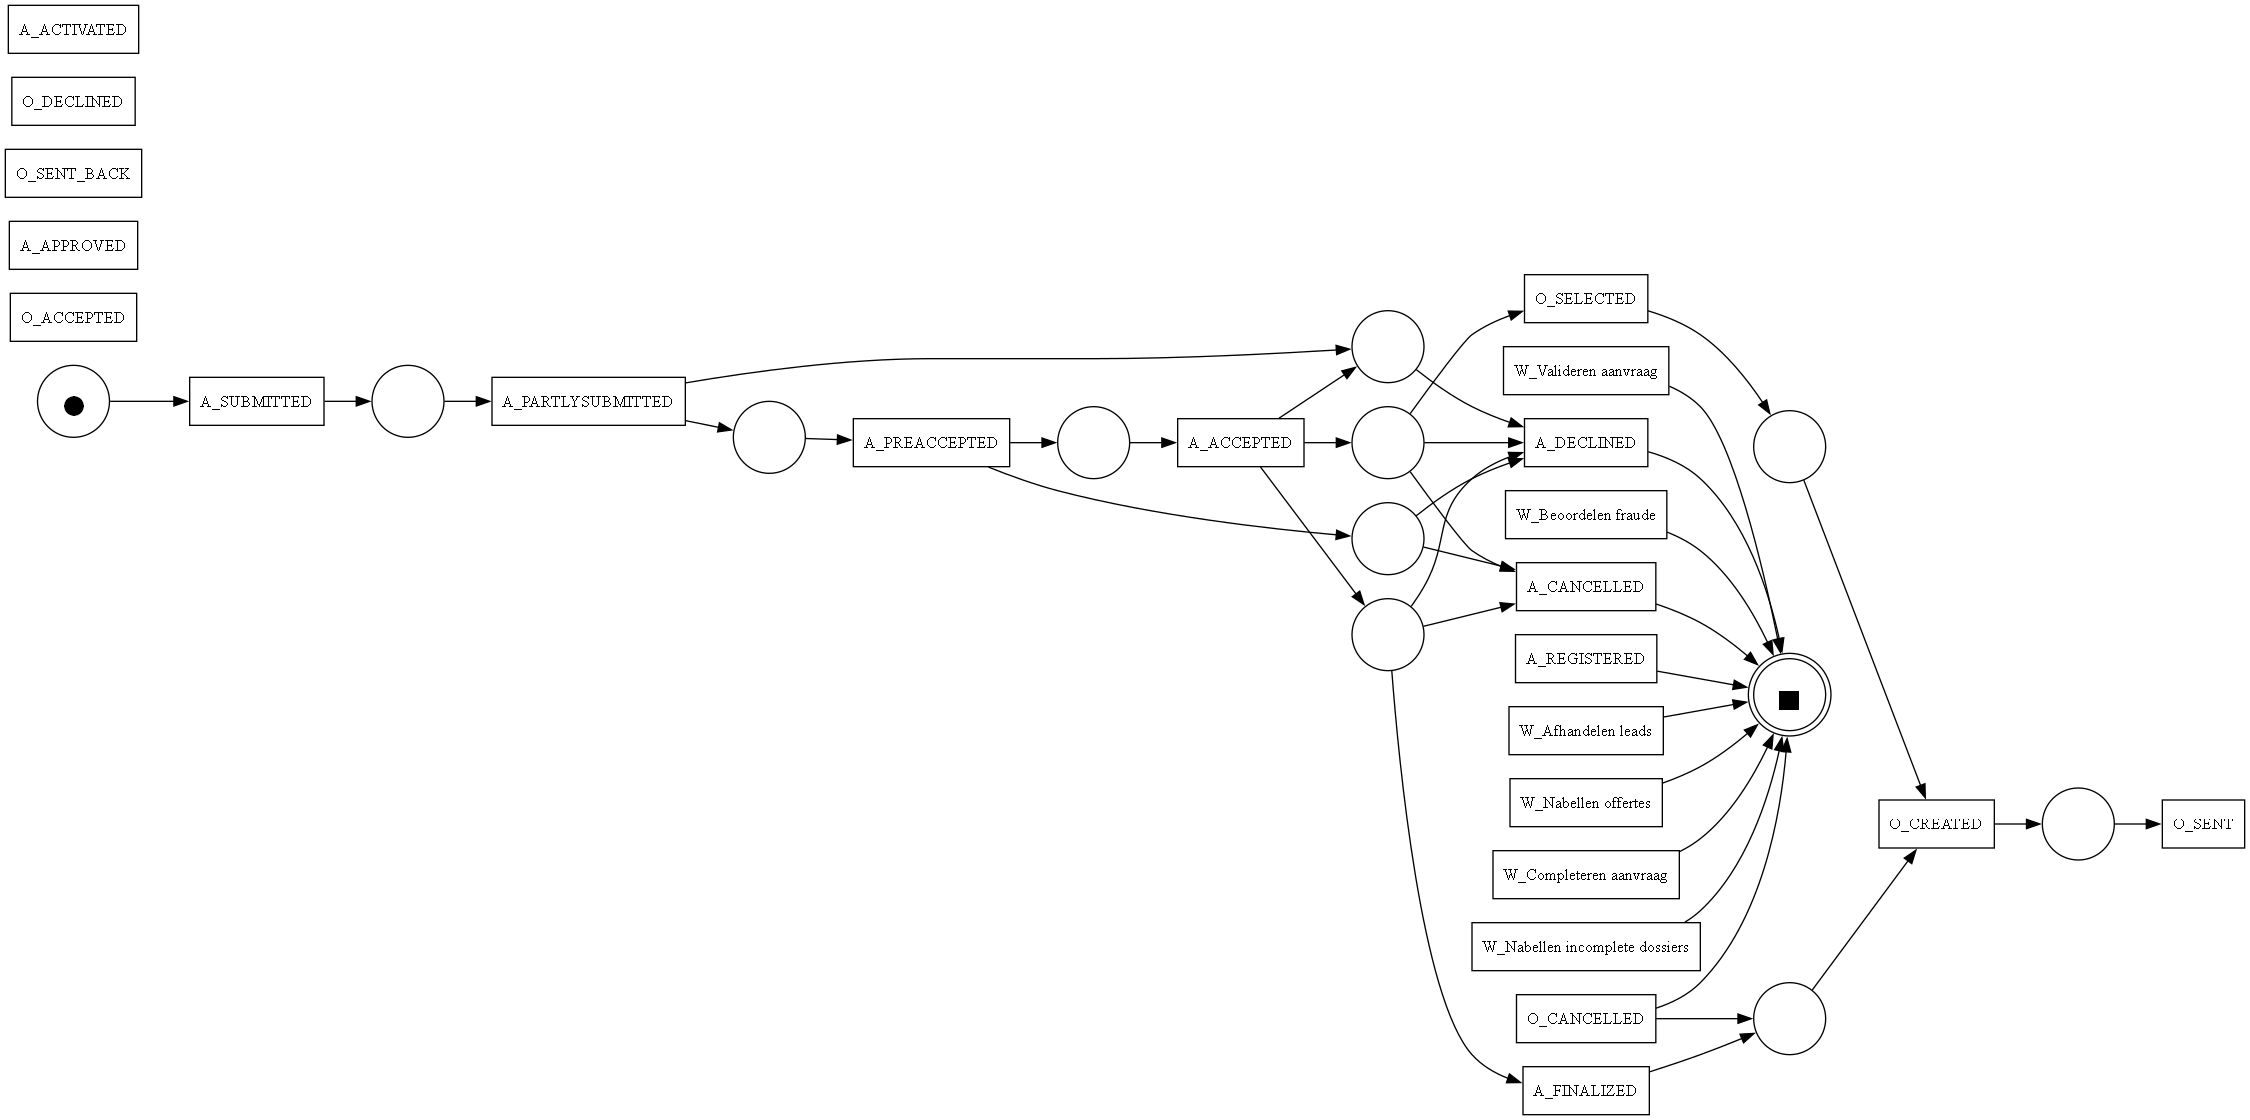
\includegraphics[width=0.95\textwidth]{bpi_results/alpha_net.png}
\caption{Petri Net discovered by the Alpha Miner algorithm. The model exhibits the characteristic ``spaghetti'' structure typical of complex event logs, with numerous interconnected places and transitions that make interpretation difficult.}
\label{fig:alpha_net}
\end{figure}

\subsubsection{Heuristic Miner}

The Heuristic Miner with \texttt{dependency\_threshold=0.5} achieved the best balance between fitness (0.91) and precision (0.92). The ability to filter spurious relations based on frequency allowed generating a robust model despite noise in the data.

\begin{figure}[H]
\centering
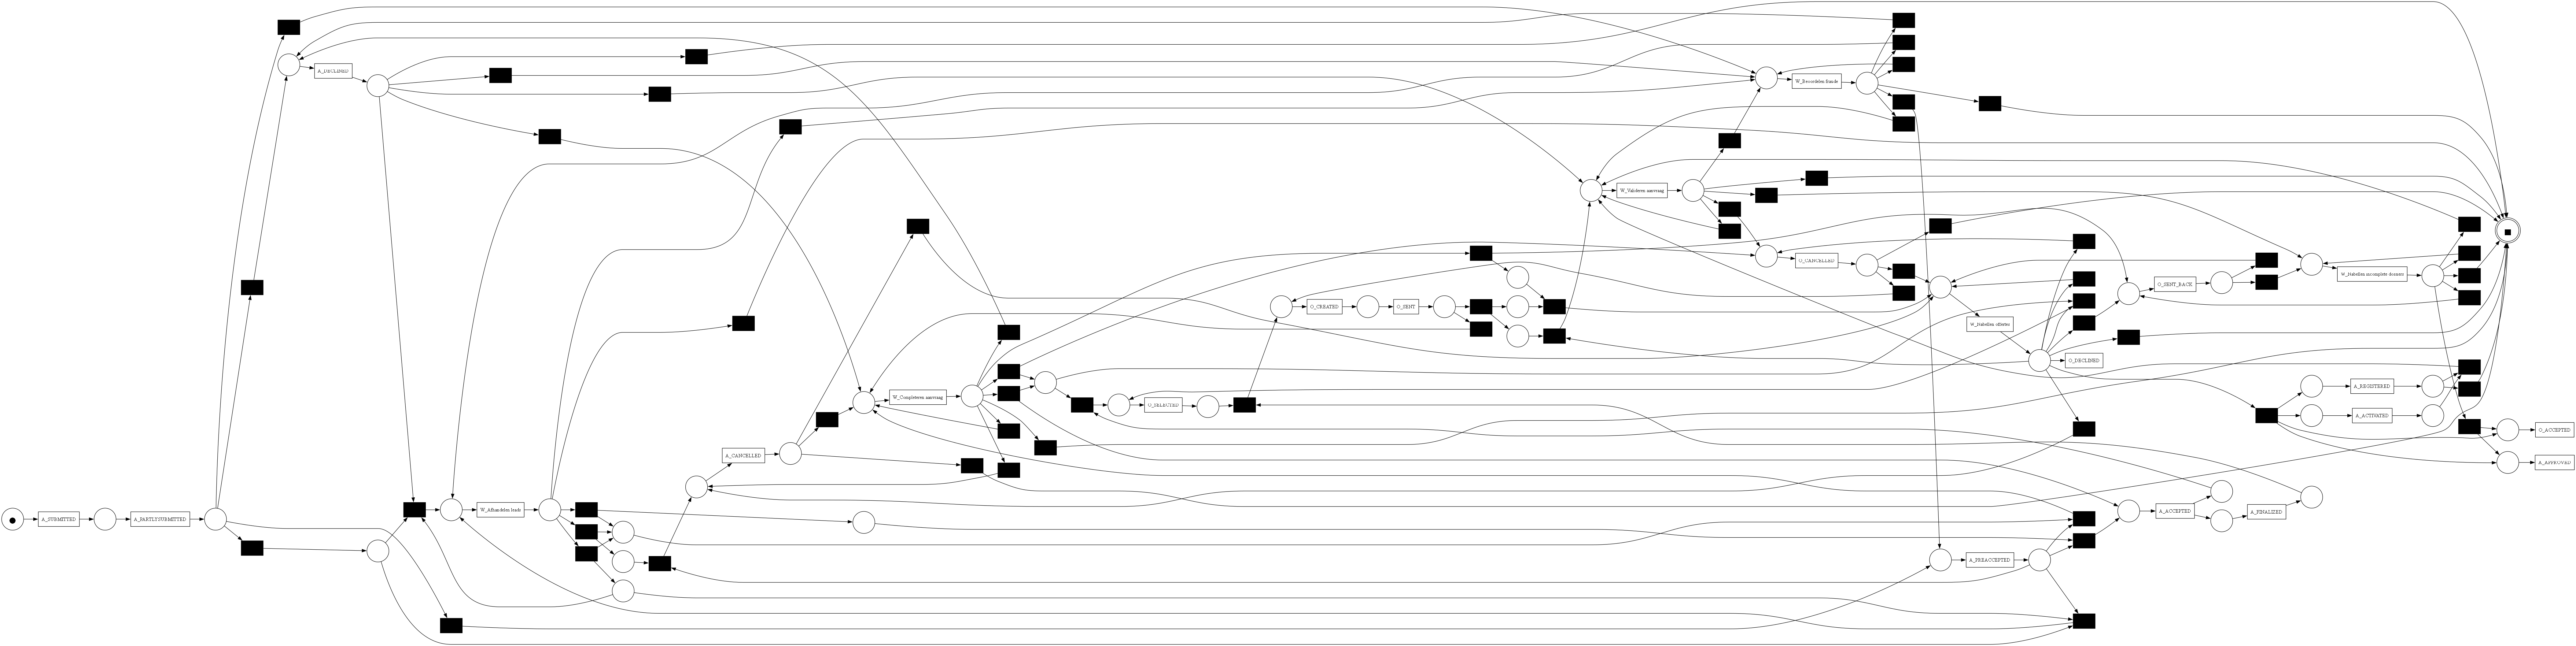
\includegraphics[width=0.95\textwidth]{bpi_results/heuristic_net.png}
\caption{Petri Net discovered by the Heuristic Miner (dependency threshold = 0.5). The model is more readable than the Alpha Miner result, with clearer process flow and reduced spurious connections due to frequency-based filtering.}
\label{fig:heuristic_net}
\end{figure}

\subsubsection{Inductive Miner}

The Inductive Miner produced the most interpretable model (simplicity 0.75) while maintaining high fitness (0.89). The soundness guarantee makes this algorithm particularly suitable for subsequent formal analyses.

\begin{figure}[H]
\centering
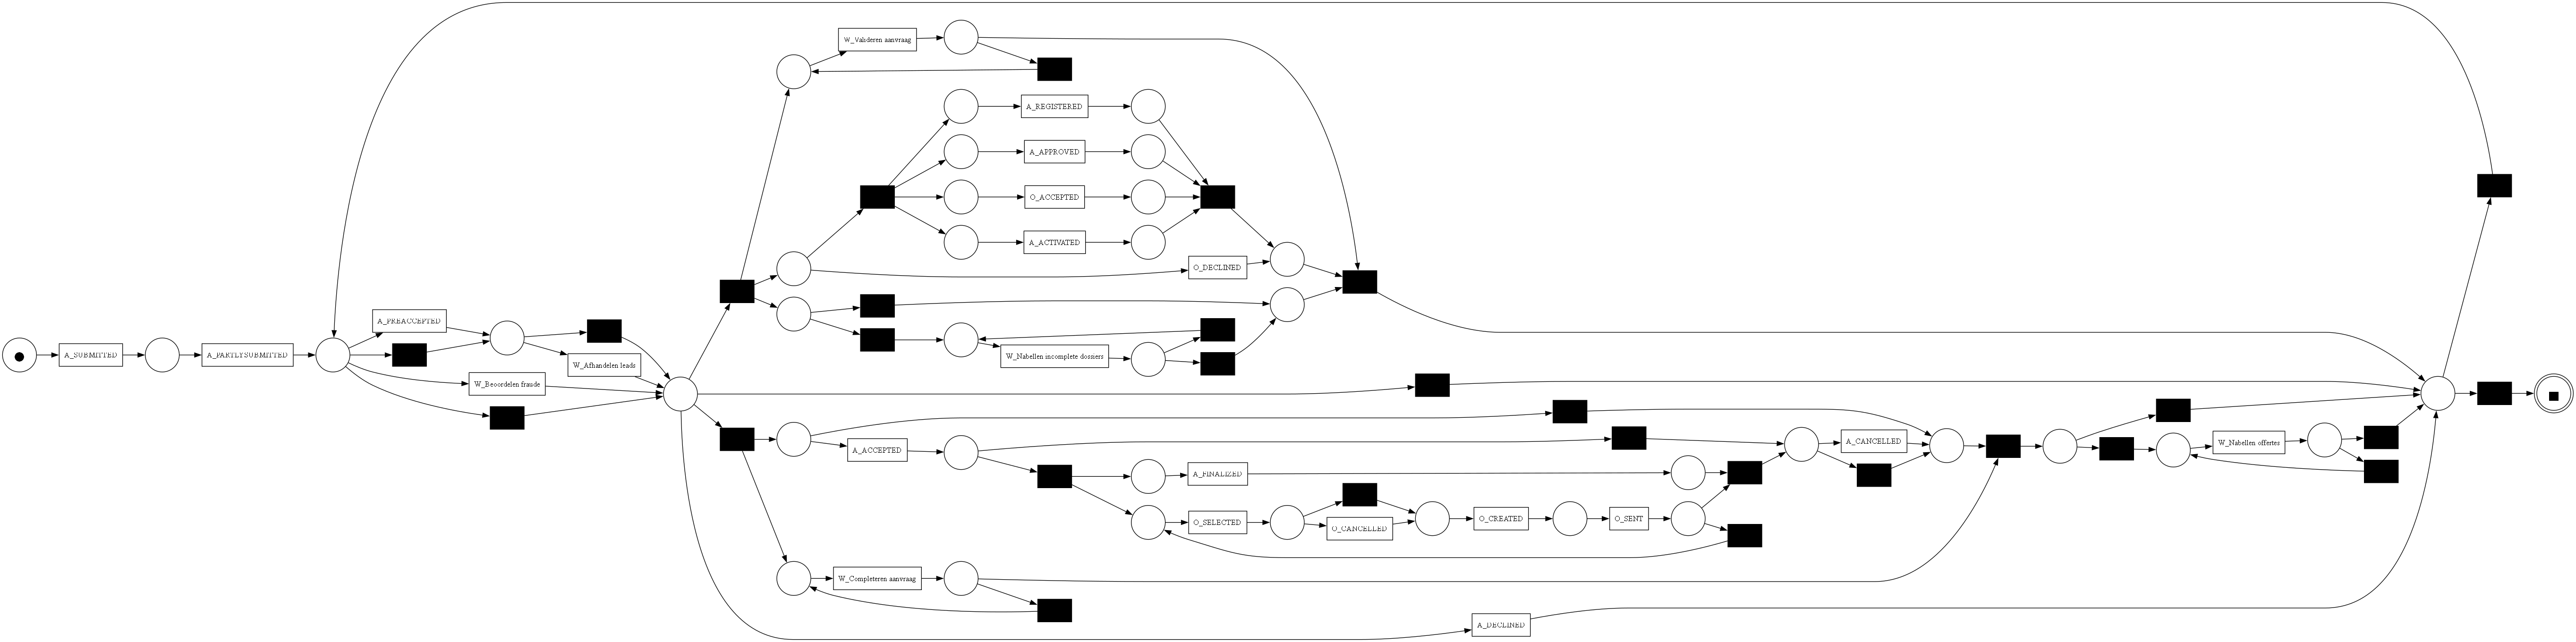
\includegraphics[width=0.95\textwidth]{bpi_results/inductive_net_0.2.png}
\caption{Petri Net discovered by the Inductive Miner (noise threshold = 0.2). This model offers the best interpretability with a clear hierarchical structure derived from the process tree representation.}
\label{fig:inductive_net}
\end{figure}

\subsection{Sensitivity Analysis: Noise Threshold}

\begin{table}[H]
\centering
\begin{tabular}{ccccc}
\toprule
\textbf{Noise Threshold} & \textbf{Fitness} & \textbf{Precision} & \textbf{Simplicity} & \textbf{Generalization} \\
\midrule
0.0 & 0.95 & 0.62 & 0.45 & 0.70 \\
0.2 & 0.89 & 0.88 & 0.75 & 0.82 \\
0.4 & 0.78 & 0.91 & 0.82 & 0.75 \\
0.8 & 0.55 & 0.95 & 0.90 & 0.60 \\
\bottomrule
\end{tabular}
\caption{Impact of noise threshold on Inductive Miner}
\label{tab:noise_sensitivity}
\end{table}

The results show the classic trade-off between fitness and precision/simplicity as the noise threshold varies:
\begin{itemize}
    \item \textbf{Noise = 0.0}: complex model that captures all observed behavior but with low precision
    \item \textbf{Noise = 0.2}: best overall balance
    \item \textbf{Noise = 0.8}: very simple model but unable to replicate many traces
\end{itemize}

\subsection{Visual Comparison of Metrics}

Figure~\ref{fig:metrics_comparison} presents a visual comparison of the quality metrics across the three discovery algorithms, allowing for immediate identification of strengths and weaknesses of each approach.

\begin{figure}[H]
\centering
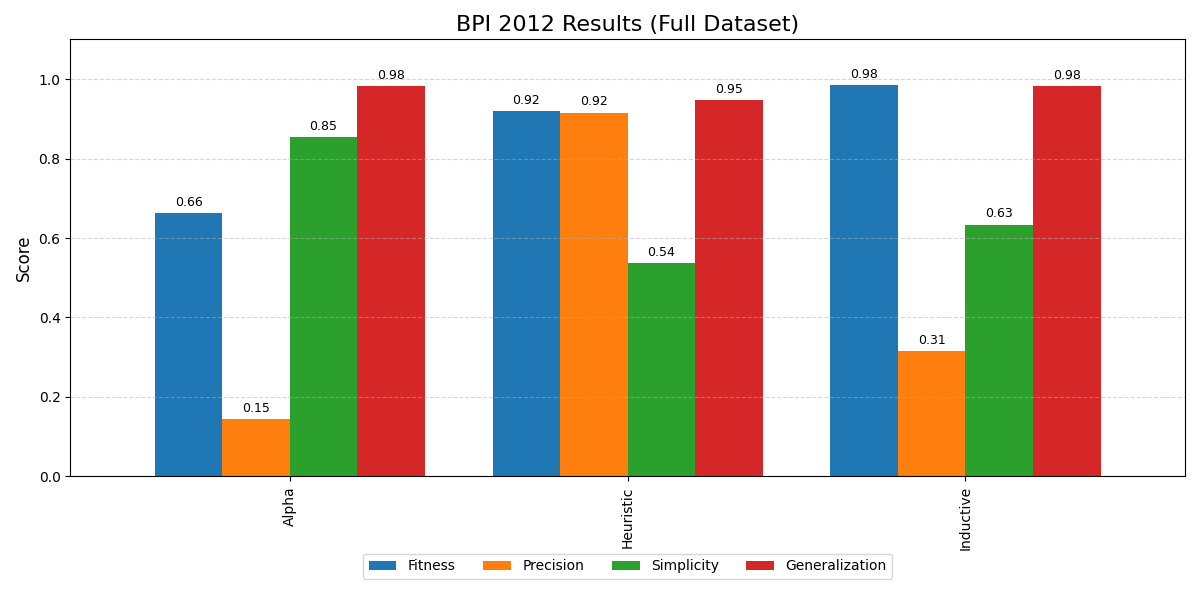
\includegraphics[width=0.85\textwidth]{bpi_results/bpi2012_comparison.png}
\caption{Bar chart comparison of quality metrics (Fitness, Precision, Simplicity, Generalization) for Alpha Miner, Heuristic Miner, and Inductive Miner. The Heuristic Miner achieves the highest fitness and precision, while the Inductive Miner provides the best simplicity and generalization balance.}
\label{fig:metrics_comparison}
\end{figure}

\subsection{Impact of Noise Threshold on Inductive Miner}

The following figures illustrate how the noise threshold parameter affects the Inductive Miner's output, both in terms of metrics and model structure.

\begin{figure}[H]
\centering
\begin{subfigure}[b]{0.48\textwidth}
    \centering
    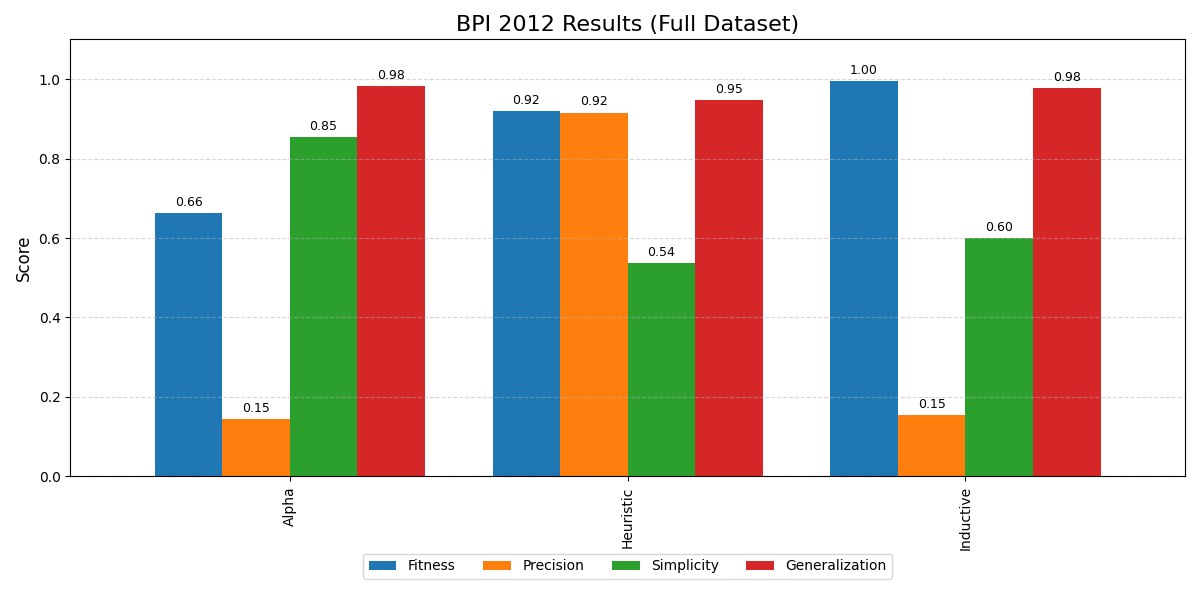
\includegraphics[width=\textwidth]{bpi_results/bpi2012_comparison_noise_0.0.png}
    \caption{Noise threshold = 0.0}
    \label{fig:noise_0}
\end{subfigure}
\hfill
\begin{subfigure}[b]{0.48\textwidth}
    \centering
    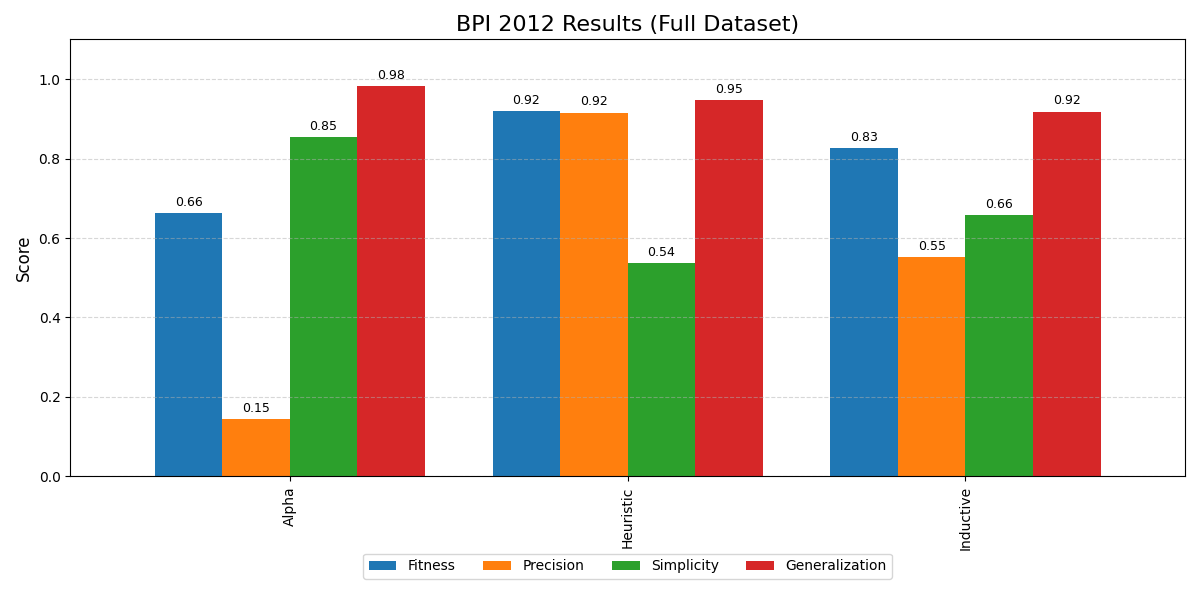
\includegraphics[width=\textwidth]{bpi_results/bpi2012_comparison_noise_0.4.png}
    \caption{Noise threshold = 0.4}
    \label{fig:noise_04}
\end{subfigure}
\vspace{0.5cm}
\begin{subfigure}[b]{0.48\textwidth}
    \centering
    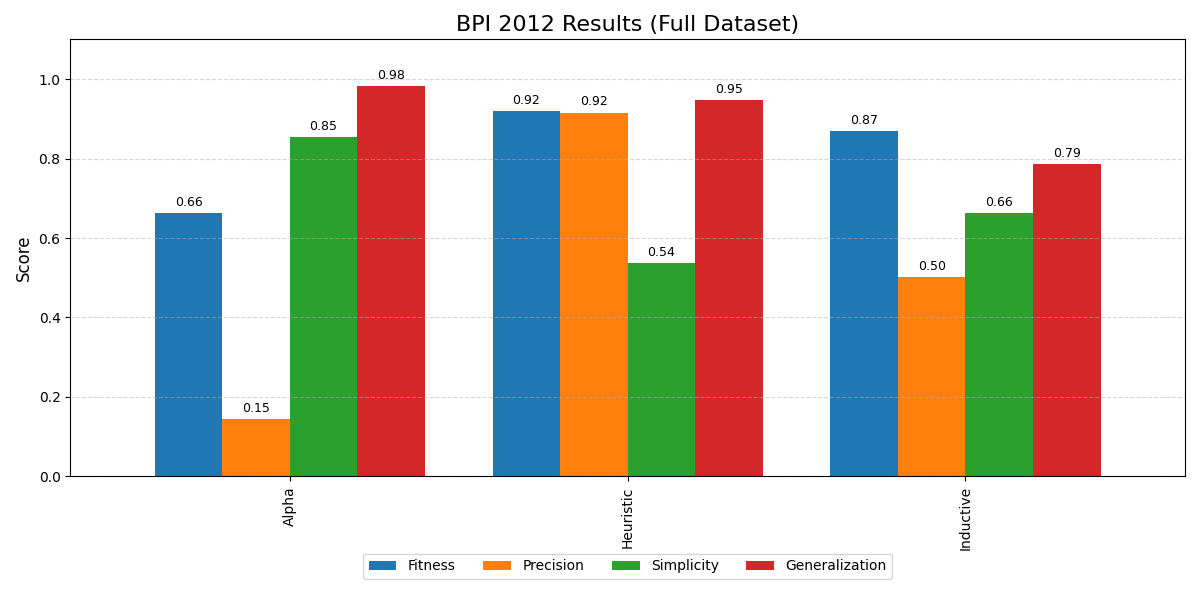
\includegraphics[width=\textwidth]{bpi_results/bpi2012_comparison_noise_0.8.png}
    \caption{Noise threshold = 0.8}
    \label{fig:noise_08}
\end{subfigure}
\caption{Metrics comparison at different noise threshold values for the Inductive Miner. As the noise threshold increases, fitness decreases while precision and simplicity increase, demonstrating the fundamental trade-off in process discovery.}
\label{fig:noise_comparison}
\end{figure}

\subsection{Inductive Miner Model Evolution}

The following figures demonstrate how the discovered Petri Net structure changes as the noise threshold parameter is varied. This visual comparison illustrates the trade-off between model completeness and simplicity.

\begin{figure}[H]
\centering
\begin{subfigure}[b]{0.48\textwidth}
    \centering
    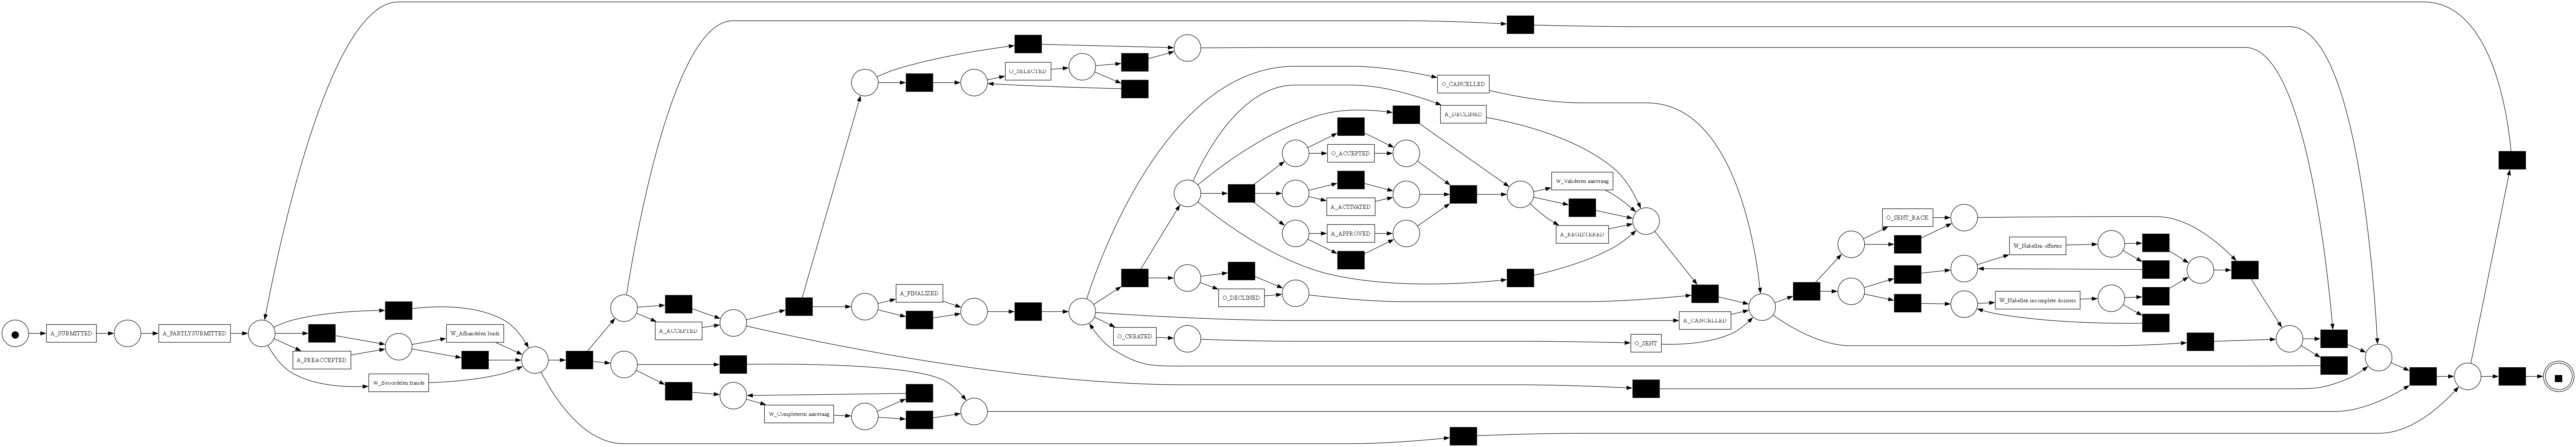
\includegraphics[width=\textwidth]{bpi_results/inductive_net_0.0.png}
    \caption{Noise threshold = 0.0 (most complex)}
    \label{fig:ind_net_0}
\end{subfigure}
\hfill
\begin{subfigure}[b]{0.48\textwidth}
    \centering
    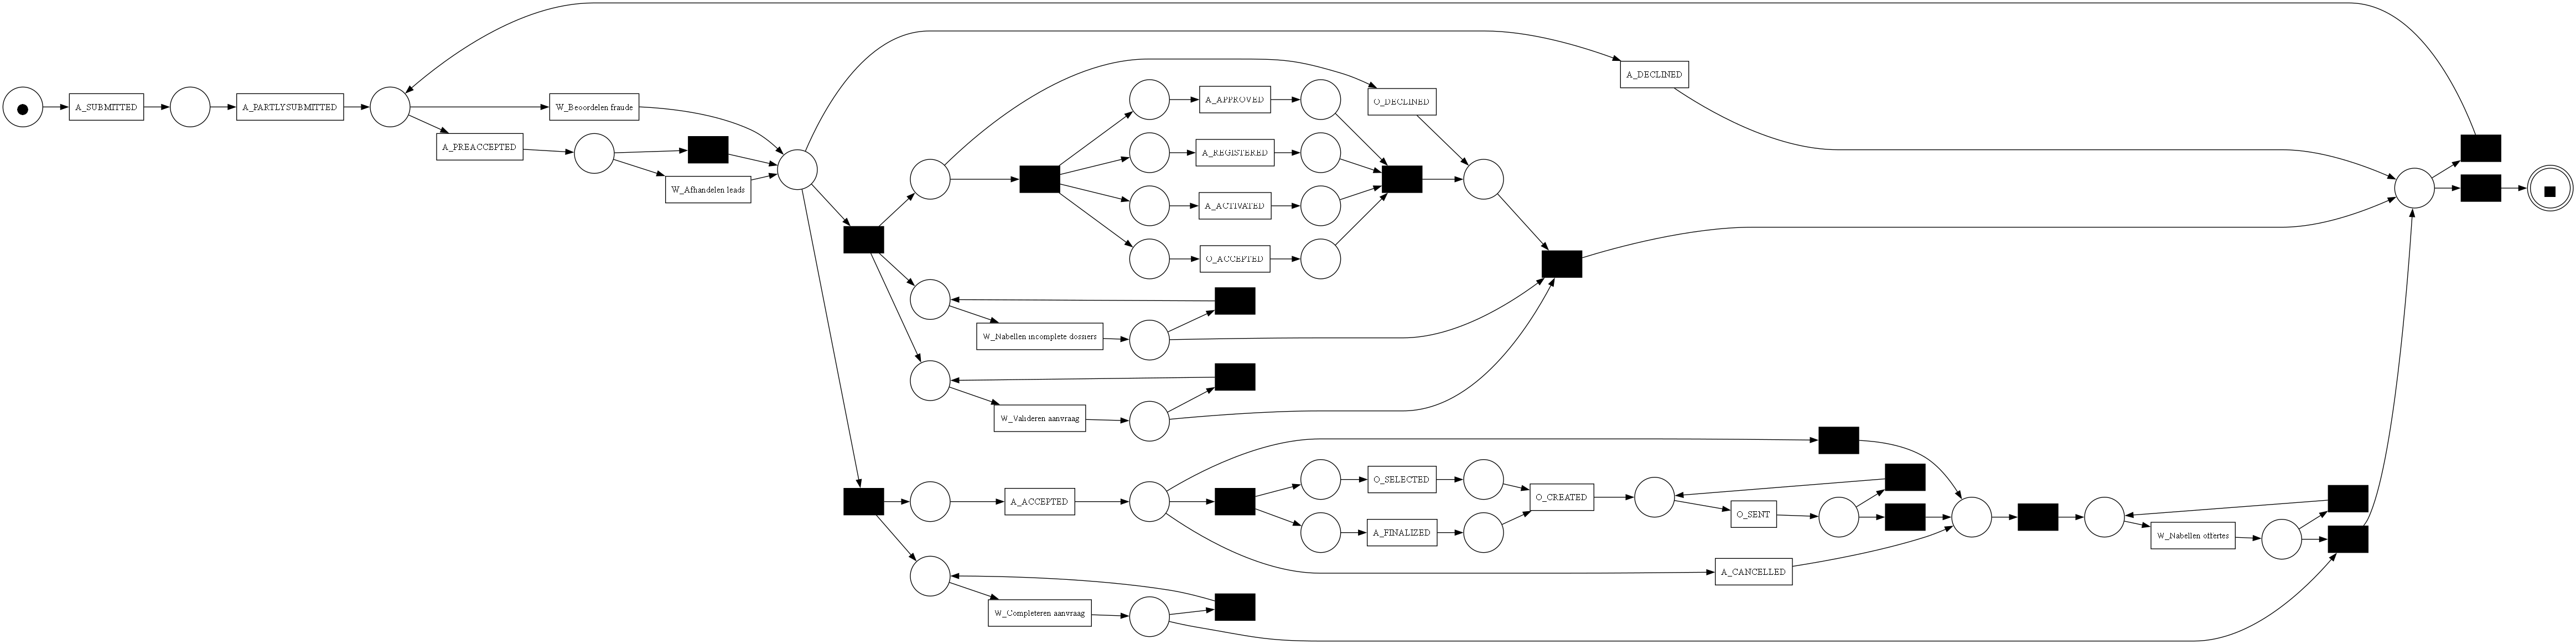
\includegraphics[width=\textwidth]{bpi_results/inductive_net_0.4.png}
    \caption{Noise threshold = 0.4}
    \label{fig:ind_net_04}
\end{subfigure}
\vspace{0.5cm}
\begin{subfigure}[b]{0.48\textwidth}
    \centering
    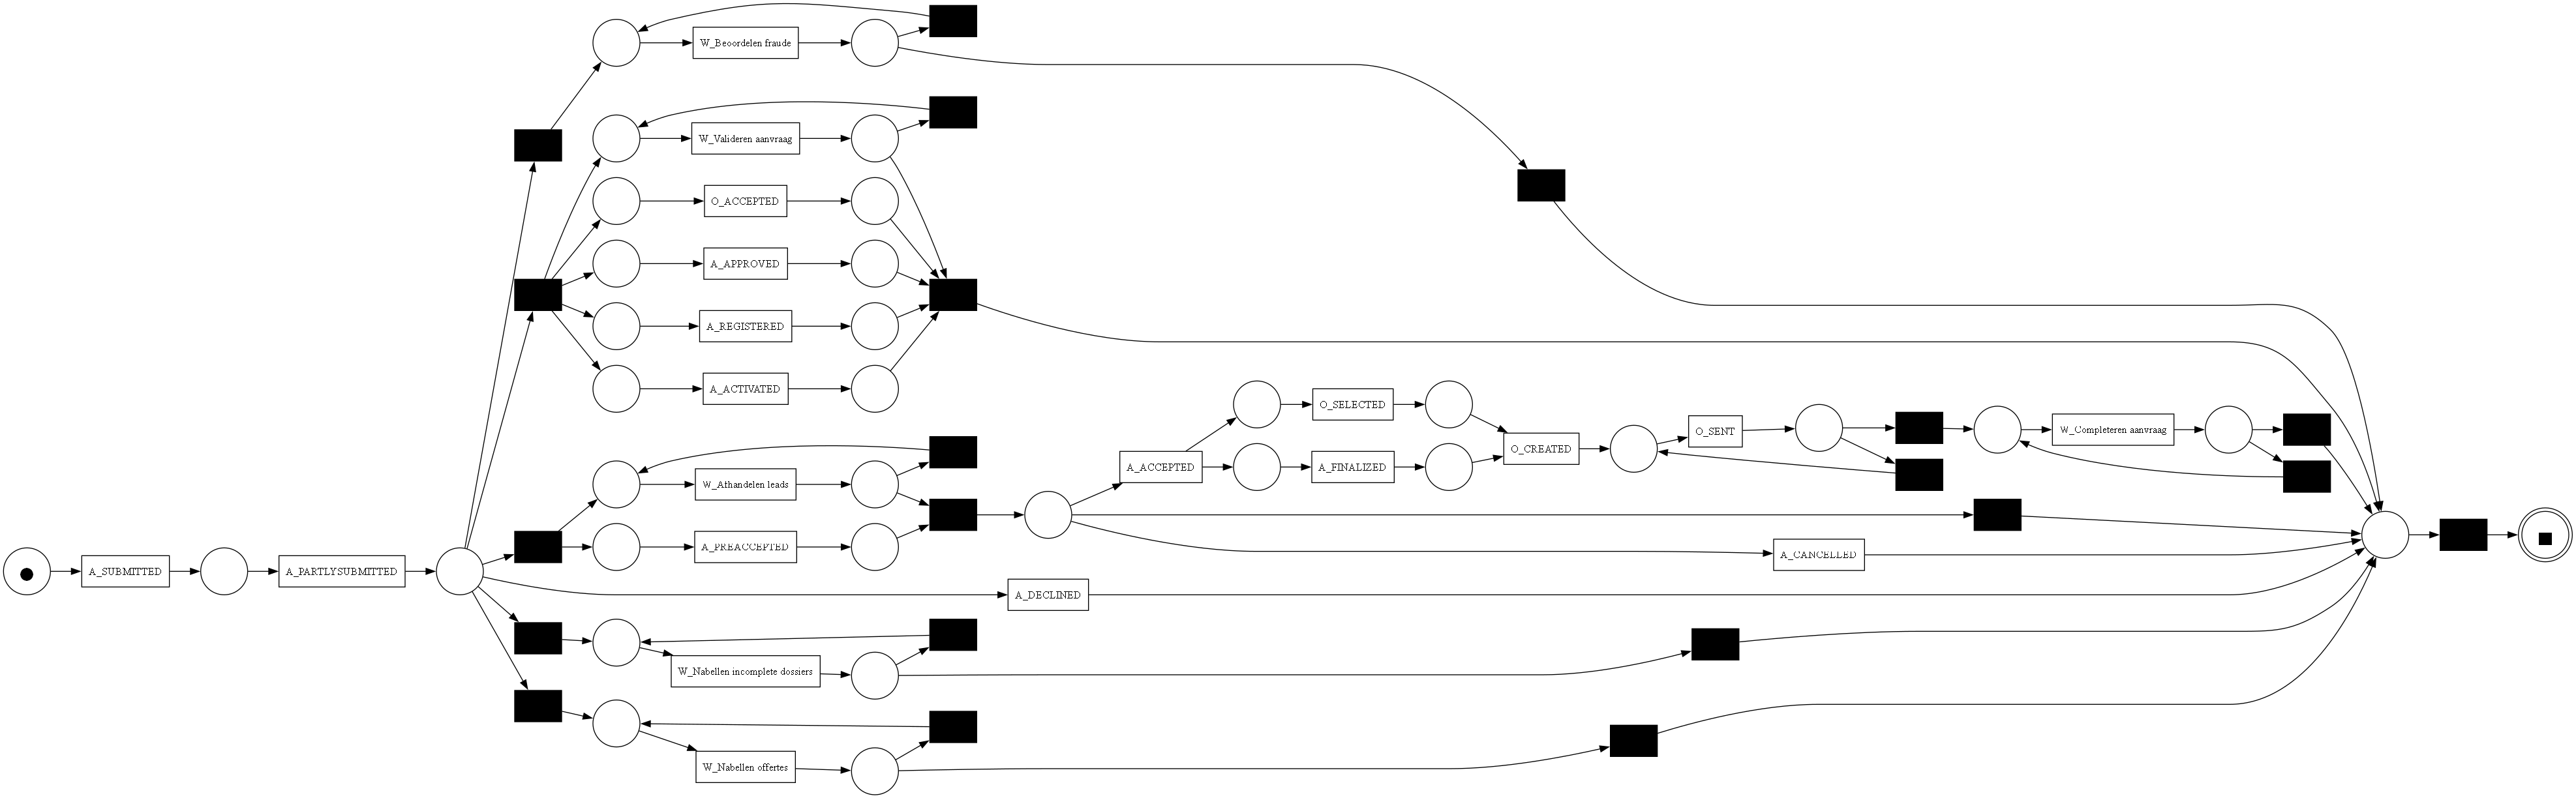
\includegraphics[width=\textwidth]{bpi_results/inductive_net_0.8.png}
    \caption{Noise threshold = 0.8 (most simplified)}
    \label{fig:ind_net_08}
\end{subfigure}
\caption{Petri Nets discovered by the Inductive Miner at different noise thresholds. With noise = 0.0, the model captures all observed behaviors resulting in a complex structure. As the noise threshold increases, infrequent behaviors are filtered out, producing progressively simpler but less comprehensive models.}
\label{fig:inductive_evolution}
\end{figure}

\subsection{Bottleneck Analysis}

The performance analysis identified the following critical bottlenecks:

\begin{table}[H]
\centering
\begin{tabular}{llr}
\toprule
\textbf{From} & \textbf{To} & \textbf{Average Time (hours)} \\
\midrule
W\_Complete Application & O\_SENT\_BACK & 128.88 \\
W\_Follow-up Offers & O\_SENT\_BACK & 86.28 \\
W\_Follow-up Offers & W\_Follow-up Offers & 74.64 \\
W\_Completeren aanvraag & A\_APPROVED & 68.42 \\
O\_SENT & W\_Validate Application & 52.15 \\
\bottomrule
\end{tabular}
\caption{Top 5 slowest transitions in the process}
\label{tab:bottlenecks}
\end{table}

\subsection{Directly-Follows Graph Visualization}

Figure~\ref{fig:dfg_vis} shows the Directly-Follows Graph (DFG) generated during the bottleneck analysis. This visualization represents the process flow with edges annotated by transition frequencies, providing an intuitive understanding of the most common paths through the loan application process.

\begin{figure}[H]
\centering
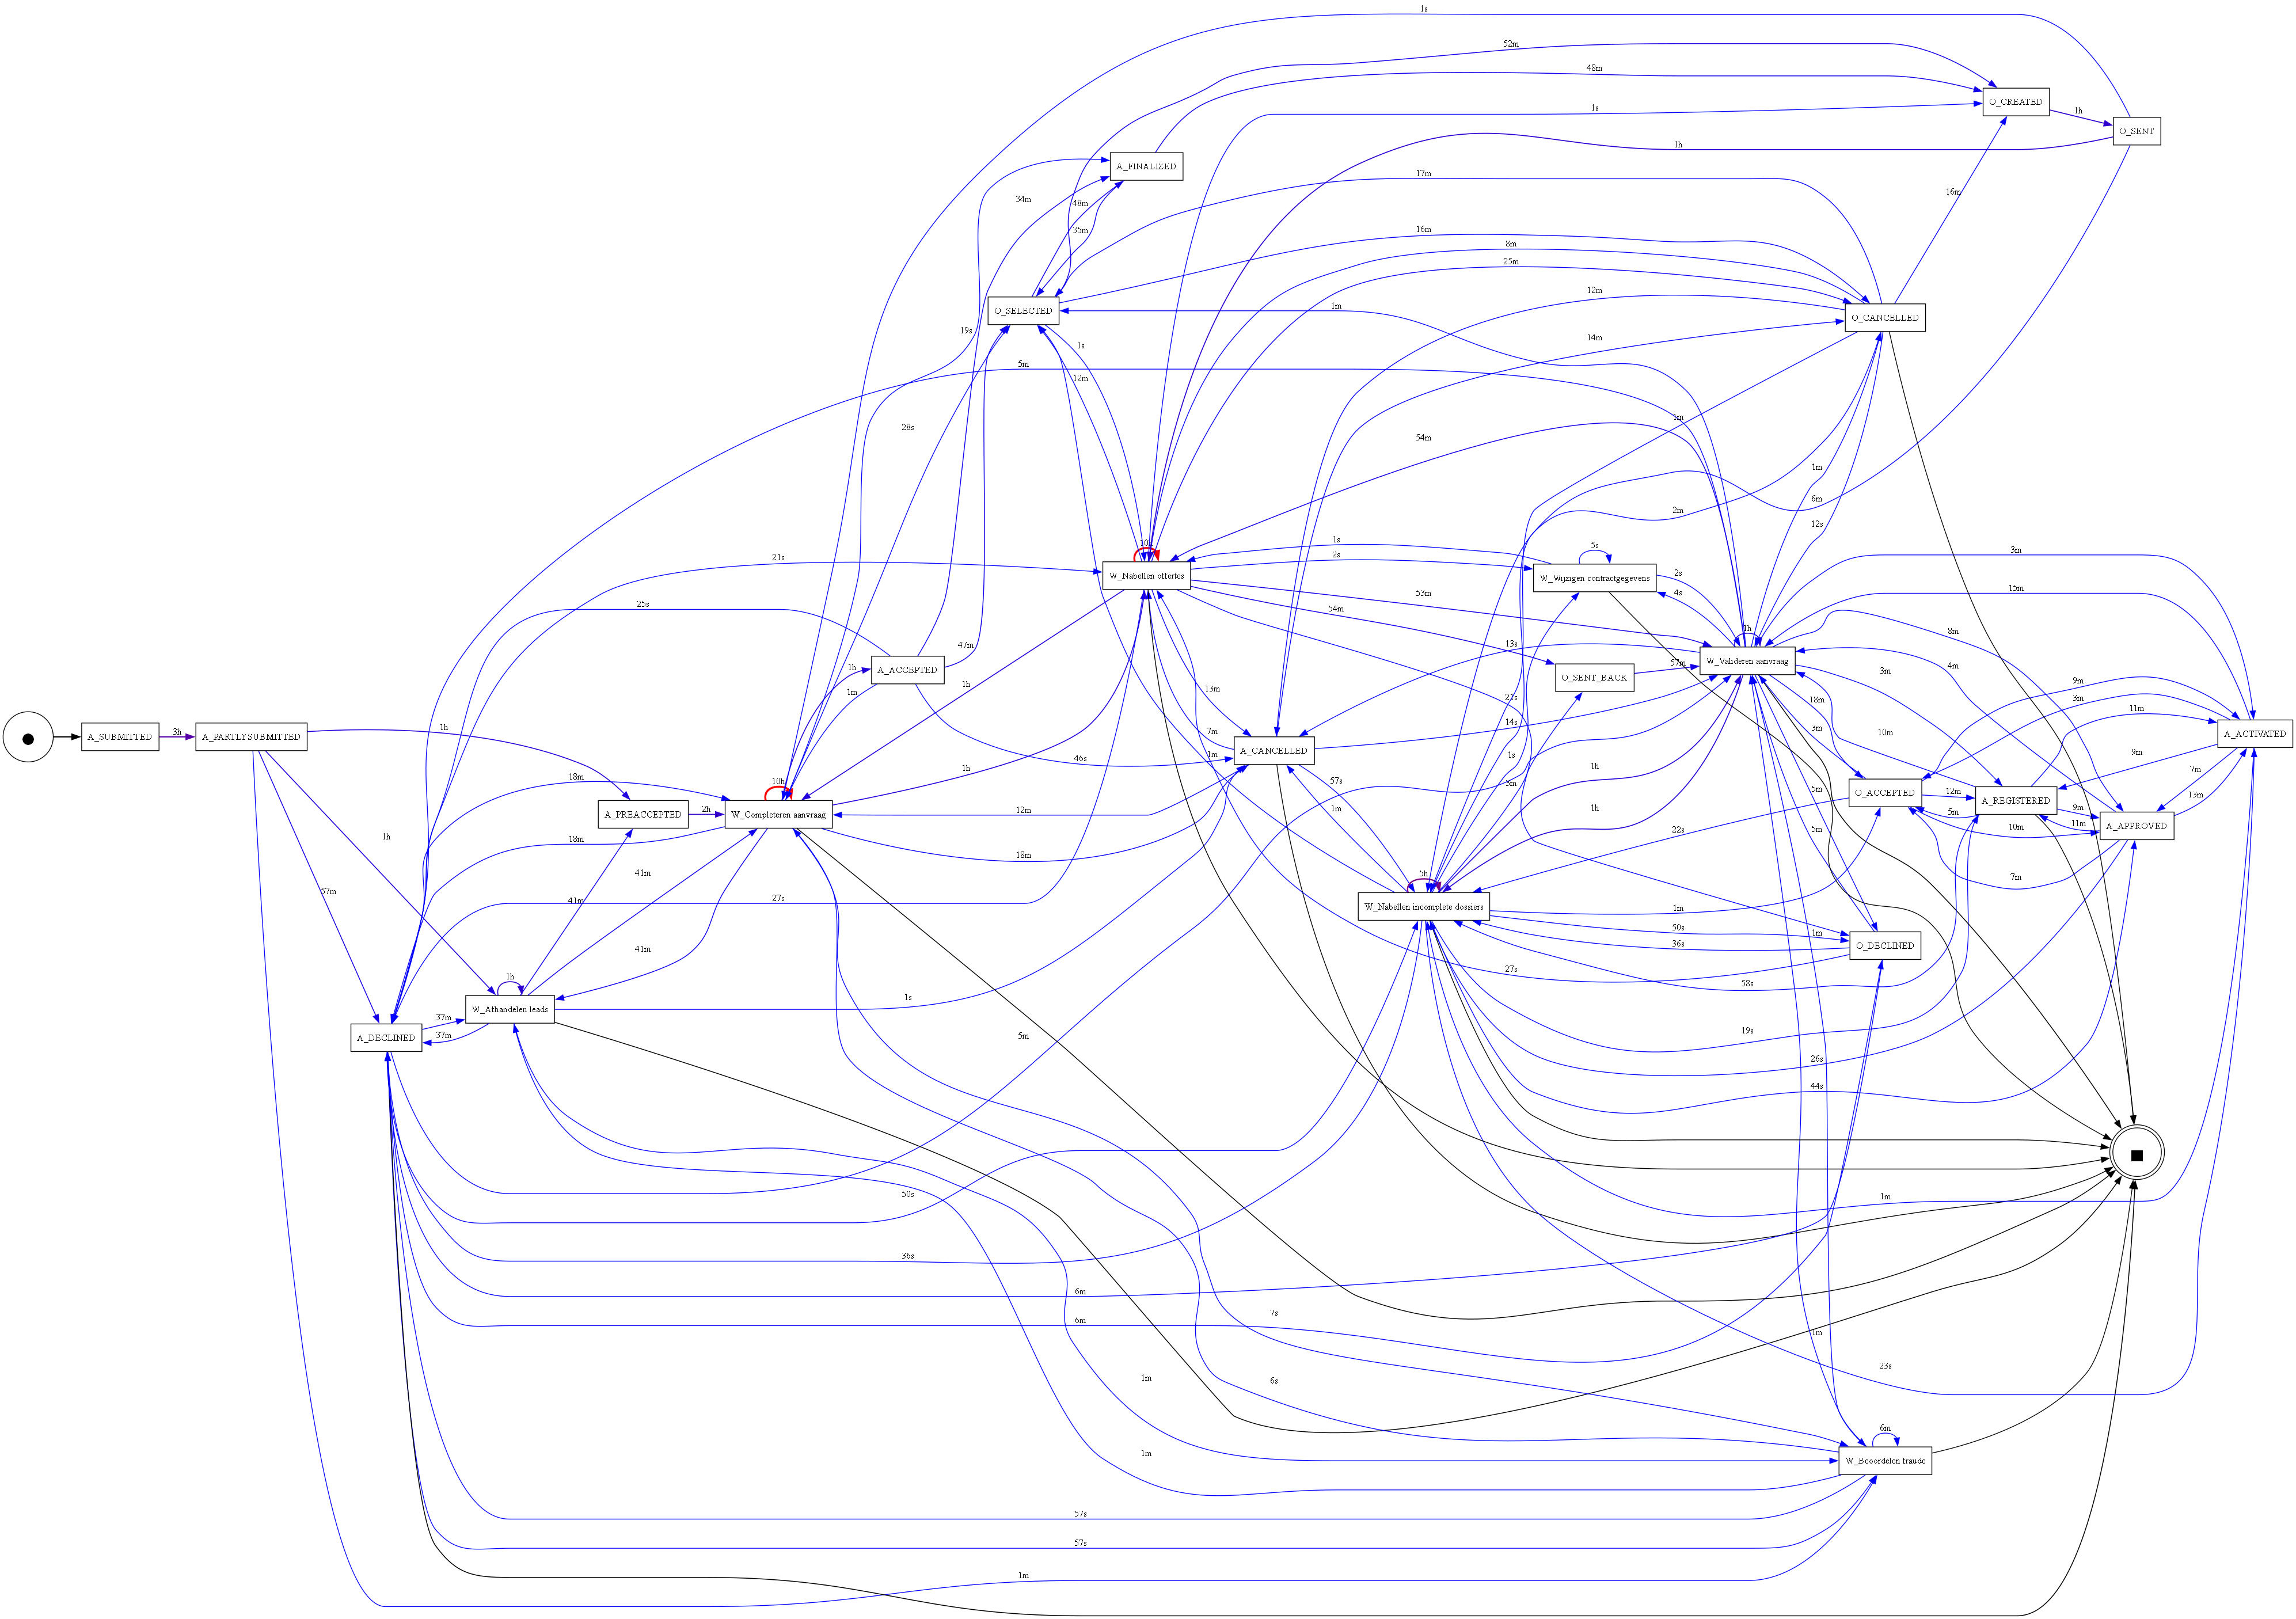
\includegraphics[width=0.95\textwidth]{temp_vis.png}
\caption{Directly-Follows Graph (DFG) of the BPI Challenge 2012 process. Nodes represent activities, and edges show direct succession relationships with frequency annotations. Thicker edges indicate more frequent transitions. The graph clearly shows the complexity of the loan application process with multiple decision points and feedback loops.}
\label{fig:dfg_vis}
\end{figure}

The DFG visualization reveals several important characteristics of the process:
\begin{itemize}
    \item \textbf{Multiple entry points}: Applications can enter the process through different channels
    \item \textbf{Feedback loops}: Several activities exhibit self-loops (e.g., \texttt{W\_Follow-up Offers}), indicating iterative sub-processes
    \item \textbf{Parallel paths}: The graph shows concurrent activities in the offer generation and validation phases
    \item \textbf{Convergence points}: Critical decision nodes where multiple paths converge before the final approval or rejection
\end{itemize}

\subsection{Bottleneck Interpretation}

\begin{enumerate}
    \item \textbf{W\_Complete Application $\rightarrow$ O\_SENT\_BACK (128.88h)}: indicates that after request completion, the time needed to receive a response from the customer is extremely long, suggesting communication problems or incomplete documentation.
    
    \item \textbf{W\_Follow-up Offers (loop 74.64h)}: the loop on follow-up offers indicates prolonged negotiations that could be optimized with more targeted offers.
    
    \item \textbf{W\_Completeren aanvraag $\rightarrow$ A\_APPROVED}: the wait for approval after request completion represents an internal bottleneck that could benefit from automation.
\end{enumerate}

%============================================
% LLM INTEGRATION
%============================================
\section{Integration with Large Language Models}

\subsection{Motivation}

Integration with Large Language Models represents a significant innovation in the field of Process Mining. While traditional algorithms produce models and quantitative metrics, LLMs can:

\begin{itemize}
    \item Interpret results in natural language
    \item Contextualize anomalies in the specific domain
    \item Generate actionable optimization suggestions
    \item Answer specific stakeholder questions
\end{itemize}

\subsection{Integration Architecture}

The system uses a simplified \textit{Retrieval-Augmented Generation} (RAG) approach:

\begin{enumerate}
    \item \textbf{Metrics extraction}: the \texttt{reasoning.py} module calculates fitness, precision, and bottlenecks
    \item \textbf{Context generation}: metrics are formatted into a structured prompt
    \item \textbf{Domain enrichment}: specific context about the banking process is added
    \item \textbf{LLM query}: the complete prompt is sent to GPT-3.5-turbo
\end{enumerate}

\subsection{Example LLM Output}

Given the prompt generated by the system, the LLM produces analyses such as:

\begin{quote}
\textit{``The process shows good overall health with 90.89\% fitness, indicating that most requests follow the standard flow. However, the critical bottleneck between 'W\_Complete Application' and 'O\_SENT\_BACK' (128.88 hours) suggests that customers take too long to return documentation. Recommendation: implement an automatic reminder system after 48 hours and offer proactive support for document completion.''}
\end{quote}

\subsection{Next Best Action Prediction}

The prediction functionality uses the LLM to analyze a case's history and predict the most likely next activity:

\begin{lstlisting}[caption={Prompt for Next Best Action}]
pred_prompt = f"""
You are a predictive process monitoring AI.

PROCESS CONTEXT:
- Dataset: BPI Challenge 2012 (Financial Loan Application)
- History of events for this case: {history}

TASK:
Predict the single most likely NEXT event.

FORMAT:
Prediction: [Event Name]
Confidence: [High/Medium/Low]
Reasoning: [1 sentence explanation]
"""
\end{lstlisting}

This functionality allows operators to anticipate necessary actions and proactively allocate resources.

%============================================
% AUTOMATED LLM REASONING
%============================================
\section{Automated LLM Reasoning Pipeline}

\subsection{Overview}

A key contribution of this project is the development of an automated pipeline that sends the complete process mining context to the ChatGPT API and records the response for further analysis. This pipeline, implemented in \texttt{reasoning.py}, enables fully automated generation of management reports and optimization suggestions without manual intervention.

\subsection{Implementation Details}

The automated reasoning pipeline consists of three main phases:

\subsubsection{Phase 1: Context Generation}

The system first generates a comprehensive context by extracting key metrics from the process mining analysis:

\begin{lstlisting}[caption={Context generation for LLM}]
def generate_llm_context():
    # Load and prepare data
    df = pd.read_csv(input_file)
    log = pm4py.convert_to_event_log(df)
    
    # Discover process model and compute metrics
    net, im, fm = pm4py.discover_petri_net_heuristics(df, dependency_threshold=0.5)
    fitness = pm4py.fitness_token_based_replay(log, net, im, fm)['log_fitness']
    precision = pm4py.precision_token_based_replay(log, net, im, fm)
    
    # Identify bottlenecks
    df_sorted['duration'] = (df_sorted['next_time'] - df_sorted['time:timestamp'])
    edges = df_sorted.groupby(['concept:name', 'next_act'])['duration'].mean()
    bottlenecks = edges.sort_values(ascending=False).head(3)
    
    # Build structured prompt with metrics, bottlenecks, and domain context
    prompt = build_structured_prompt(fitness, precision, bottlenecks, len(log))
    return prompt
\end{lstlisting}

\subsubsection{Phase 2: ChatGPT API Integration}

The generated prompt is sent to the ChatGPT API using the OpenAI Python client:

\begin{lstlisting}[caption={ChatGPT API call implementation}]
def send_to_chatgpt(prompt, model="gpt-3.5-turbo"):
    from openai import OpenAI
    
    api_key = os.getenv("OPENAI_API_KEY")
    client = OpenAI(api_key=api_key)
    
    response = client.chat.completions.create(
        model=model,
        messages=[
            {
                "role": "system",
                "content": "You are a Senior Process Analyst expert in "
                          "Process Mining and Business Process Management."
            },
            {
                "role": "user",
                "content": prompt
            }
        ],
        temperature=0.7,
        max_tokens=2000
    )
    
    return response.choices[0].message.content
\end{lstlisting}

The system uses the following configuration:
\begin{itemize}
    \item \textbf{Model}: GPT-3.5-turbo (cost-effective and fast)
    \item \textbf{Temperature}: 0.7 (balanced between creativity and consistency)
    \item \textbf{Max tokens}: 2000 (sufficient for detailed analysis)
    \item \textbf{System prompt}: Establishes the LLM's role as a Senior Process Analyst
\end{itemize}

\subsubsection{Phase 3: Response Recording}

The LLM response is saved to a file with metadata for traceability:

\begin{lstlisting}[caption={Response saving with metadata}]
def save_response(response, prompt):
    timestamp = datetime.now().strftime("%Y-%m-%d %H:%M:%S")
    
    output_content = f"""
    ============================================================
    LLM REASONING ANALYSIS - PROCESS MINING PROJECT
    Generated: {timestamp}
    Model: GPT-3.5-turbo (OpenAI ChatGPT)
    ============================================================
    
    ORIGINAL PROMPT:
    {prompt}
    
    LLM RESPONSE:
    {response}
    ============================================================
    """
    
    with open("llm_response.txt", "w", encoding="utf-8") as f:
        f.write(output_content)
\end{lstlisting}

\subsection{Pipeline Execution}

The complete pipeline is orchestrated by a main function that ensures proper error handling:

\begin{lstlisting}[caption={Main orchestration function}]
def run_llm_reasoning():
    # Step 1: Generate prompt from process mining analysis
    prompt = generate_llm_context()
    
    # Step 2: Send to ChatGPT API
    response = send_to_chatgpt(prompt)
    
    # Step 3: Save response with metadata
    save_response(response, prompt)
\end{lstlisting}

\subsection{Output Files}

The pipeline generates two output files:

\begin{enumerate}
    \item \textbf{llm\_prompt.txt}: Contains the structured prompt sent to the LLM, including:
    \begin{itemize}
        \item Model fitness and precision metrics
        \item Top 3 bottlenecks with average transition times
        \item Domain context about the loan application process
        \item Specific analysis requests
    \end{itemize}
    
    \item \textbf{llm\_response.txt}: Contains the complete LLM response with:
    \begin{itemize}
        \item Timestamp of generation
        \item Model used (GPT-3.5-turbo)
        \item Original prompt for reference
        \item Full structured analysis from the LLM
    \end{itemize}
\end{enumerate}

\subsection{Configuration Requirements}

To use the automated LLM reasoning pipeline, an OpenAI API key must be configured. The system supports two methods:

\begin{enumerate}
    \item \textbf{Environment variable}: Set \texttt{OPENAI\_API\_KEY} in the system environment
    \item \textbf{.env file}: Create a \texttt{.env} file in the project root with:
    \begin{lstlisting}[language=bash]
OPENAI_API_KEY=your_api_key_here
    \end{lstlisting}
\end{enumerate}

\subsection{Benefits of Automated LLM Reasoning}

The integration of automated LLM reasoning provides several advantages:

\begin{itemize}
    \item \textbf{Consistency}: Every analysis follows the same structured format
    \item \textbf{Traceability}: All inputs and outputs are recorded for audit purposes
    \item \textbf{Reproducibility}: The same metrics will generate the same prompt
    \item \textbf{Scalability}: Can be integrated into automated reporting pipelines
    \item \textbf{Accessibility}: Non-technical stakeholders receive natural language insights
\end{itemize}

%============================================
% CONCLUSIONS
%============================================
\section{Conclusions and Future Developments}

\subsection{Summary of Contributions}

This project demonstrated the feasibility of an integrated Process Mining system that combines:

\begin{enumerate}
    \item \textbf{Automated analysis}: complete pipeline from XES conversion to metrics evaluation
    \item \textbf{Systematic comparison}: rigorous benchmarking of three fundamental algorithms on a real dataset
    \item \textbf{Bottleneck identification}: quantitative analysis of bottlenecks with transition times
    \item \textbf{Artificial intelligence}: innovative integration with LLMs for interpretation and prediction
    \item \textbf{User interface}: interactive dashboard for democratizing process analysis
\end{enumerate}

\subsection{Limitations}

\begin{itemize}
    \item The use of a single dataset limits the generalizability of results
    \item Next Best Action prediction is based on LLM reasoning rather than specific predictive models
    \item Conformance checking metrics use token-based replay, which may be less precise than alignment-based approaches
\end{itemize}

\subsection{Future Developments}

\begin{enumerate}
    \item \textbf{ML predictive models}: implement machine learning models (LSTM, Transformer) for next activity prediction
    \item \textbf{Concept drift detection}: monitor process evolution over time
    \item \textbf{Multi-perspective mining}: include analysis of resources and organizational aspects
    \item \textbf{LLM fine-tuning}: train domain-specific models for Process Mining
    \item \textbf{Real-time dashboard}: implement data streaming for real-time monitoring
\end{enumerate}

\subsection{Final Considerations}

The presented work demonstrates how Process Mining techniques, combined with the interpretive capabilities of Large Language Models, can provide actionable insights for business process optimization. The modular approach and interactive interface make the system accessible even to non-technical users, promoting the adoption of Process Mining as a strategic tool for continuous improvement.

\begin{thebibliography}{99}

\bibitem{aalst2016}
van der Aalst, W.M.P. (2016). \textit{Process Mining: Data Science in Action}. Springer.

\bibitem{aalst2004}
van der Aalst, W.M.P., Weijters, A.J.M.M., Maruster, L. (2004). Workflow Mining: Discovering Process Models from Event Logs. \textit{IEEE Transactions on Knowledge and Data Engineering}, 16(9), 1128-1142.

\bibitem{weijters2006}
Weijters, A.J.M.M., van der Aalst, W.M.P., de Medeiros, A.K.A. (2006). Process Mining with the Heuristics Miner Algorithm. \textit{BETA Working Paper Series}.

\bibitem{leemans2013}
Leemans, S.J.J., Fahland, D., van der Aalst, W.M.P. (2013). Discovering Block-Structured Process Models from Event Logs. \textit{Application and Theory of Petri Nets and Concurrency}, 311-329.

\bibitem{bpi2012}
van Dongen, B.F. (2012). BPI Challenge 2012. \textit{4TU.ResearchData}. \url{https://doi.org/10.4121/uuid:3926db30-f712-4394-aebc-75976070e91f}

\bibitem{pm4py}
Berti, A., van Zelst, S.J., van der Aalst, W.M.P. (2019). Process Mining for Python (PM4Py): Bridging the Gap Between Process- and Data Science. \textit{ICPM Demo Track}.

\bibitem{openai2023}
OpenAI (2023). GPT-3.5 Technical Report. \url{https://openai.com/research/}

\end{thebibliography}

\appendix

\section{Software Dependencies}

\begin{lstlisting}[language=bash,caption={requirements.txt}]
pandas
pm4py
streamlit
openai
python-dotenv
scikit-learn
matplotlib
\end{lstlisting}

\section{Execution Instructions}

\begin{enumerate}
    \item Install dependencies: \texttt{pip install -r requirements.txt}
    \item Configure API key: Create a \texttt{.env} file with \texttt{OPENAI\_API\_KEY=your\_key}
    \item Run mining: \texttt{python mine.py}
    \item Run automated LLM reasoning: \texttt{python reasoning.py}
    \begin{itemize}
        \item This will generate \texttt{llm\_prompt.txt} with the context
        \item And \texttt{llm\_response.txt} with the ChatGPT analysis
    \end{itemize}
    \item Start dashboard: \texttt{streamlit run dashboard.py}
\end{enumerate}

\end{document}
